\documentclass{article}
\usepackage{url}
\usepackage{graphicx}
\usepackage{amssymb}
\usepackage{amsmath}
\usepackage{geometry}
\usepackage{cite}
\usepackage{hyperref} % Nice details for pdf


\geometry{
	verbose,
	letterpaper,
	tmargin=3cm,
	bmargin=3cm,
	lmargin=2cm,
	rmargin=2cm
}

\hypersetup{
	bookmarksopen=true,
	colorlinks=true,
	linkcolor=blue,
	citecolor=blue,
	urlcolor=black,	
	linktoc=all,
	pdftitle={FEM Simulation of Normal Modes of Vibration in a Colombian Andean Bandola in C},
	pdfauthor={S. Gomez, N. Guarin-Zapata},
	pdfkeywords={Bandola, Musical Acoustics, Computational Mechanics, Finite Element Methods},
	pdfsubject={FEA for Andean Bandola},
	pdfpagemode=UseOutlines,
	pdfstartview=FitH
}

\begin{document}


\title{\textbf{FEM Simulation of Normal Modes of Vibration in a Colombian Andean Bandola in C}}

\author{Sara E. Rodr\'iguez G\'omez and Nicol\'as Guar\'in--Zapata}


\maketitle

\begin{abstract}
Musical acoustics have emerged as a branch that studies the sound produced for musical purposes. The specific subject of acoustics of strings instruments like guitar and violin has been extensively treated and important results of modal analysis at low resonances have shown the Fluid-structure coupling at its first two and three resonances \cite{Hutchins, Firth1, Christensen, Christensen3, Elejabarrieta} where commonly the instruments range of pitch is covered. The response at these resonances becomes important to study the sound quality of instruments; therefore, many reported models have related uncoupled modes of the air inside the acoustic box and top/back plates with the assembled instruments modes. In order to begin to understand the acoustical operation, we analyze the dynamical behavior of a ``drop shaped'' Colombian stringed instrument -the ``Bandola Andina''- at low resonances by the FEM and the coupling phenomenon is verified through the model used in \cite{Christensen, Christensen3}.

\end{abstract}

\textbf{Keyword:} Musical Acoustics, Modal Analysis, Finite Element Method, Stringed Instruments, Bandola.


\section{Introduction}

Research on the acoustics of musical instruments, a field named musical acoustics, has attempted to relate physical parameters with the characteristic sound of an instrument \cite{Caldersmith1, Christensen, Christensen3, Dickens1, Firth1, Rossing, Rossing1, Rossing3, Jannsson, Jansson:GuitarModes, Knotta, Marshall, Meyer, Meyer2, Boullosa, Richardson, Molin, Stetson, Woodhouse, J.Torres1, J.Torres, Elejabarrieta, French, Boullosa1, Boullosa2, Caldersmith, Hutchins}. For this purpose, some phenomena, mainly in the sound production and propagation, are studied based on the behavior of the instrument. The first important application of musical acoustics was done to violins and guitars \cite{Caldersmith1, Christensen, Christensen3, Dickens1, Firth1, Rossing, Rossing1, Rossing3, Jannsson, Jansson:GuitarModes, Knotta, Marshall, Meyer, Meyer2, Boullosa, Richardson, Molin, Stetson, Woodhouse, J.Torres1, J.Torres, Elejabarrieta, French, Boullosa1, Boullosa2, Caldersmith, Hutchins}, the study of these instruments provided useful information to luthiers about parameters that could modify the acoustical response of the instrument. In this sense, this work studies, using the finite element method, the normal modes of vibration for the Colombian Andean C-Bandola.

The Colombian Andean Bandola is a musical instrument that experienced a parallel development in many places and which currently presents different regionalized design adaptations. Given these conditions, it is not possible to identify a standard Colombian Andean Bandola, not even a single characteristic sound or tuning \cite{thesis:bandola}. The differences lie in the ways in which instruments are built by regional luthiers and this fact, together with reforms recently proposed by musicians and luthiers from Bogota savannah, have led to a discussion about the identity of the instrument with respect to its sonority and national musical tradition \cite{thesis:bandola}.

Normal modes are well known acoustic parameters which describe the vibrational response of the instrument. The bandola could be understood as a complex mechanical system, whose dynamic behavior depends largely on the interaction and coupling of each of its constituent elements. Knowledge about the dynamic characteristics of resonance box elements can give an idea of how structural parameters influence the behavior of the instrument as a whole. The analysis of modal coupling at the resonance box is thus proposed and developed throughout the document. 

The methodology and results were validated based on reported studies, primarily of guitars. The analysis at low resonances is emphasized through two models consisting of coupled oscillators, which could represent the vibrations of enclosed air, top and back plates at their lowest resonances. The approach of a project on this topic is intended not only contributions in academia, but also potential cultural impacts.

\section{The Colombian Andean Bandola and its analysis}

Colombian Andean Bandola is a plucked string instrument that comes from guitar family. Its name comes from an old persian-arabic root, pandur, that comes through different north african and european instruments and indicates a variety of melodic instruments with high and medium pitch. This instrument presents several design adaptations through history in different Colombian regions that differ essentially in dimensions, process of building and tuning. Bandola in C (tuned in C) and bandola in B$\flat$ (tuned in B$\flat$) are the most representative prototypes.

The analysis proposed in this document is considered for bandola in C, which has been accepted and markedly used in last years by \textit{estudiantinas} (musical groups similar to Tunas). Hence, following descriptions pertain to this instrument with C-tuning. The bandola in C presents twelve strings grouped in unison pairs. Strings form six groups tuned in intervals of perfect fourths \cite{thesis:bandola}. Figure \ref{Bandola} presents the bandola and the pitchs for each string. The frequency values that correspond to the tuning of each open string are specified in Table \ref{StringTuning}.

\begin{figure}[h]
\centering
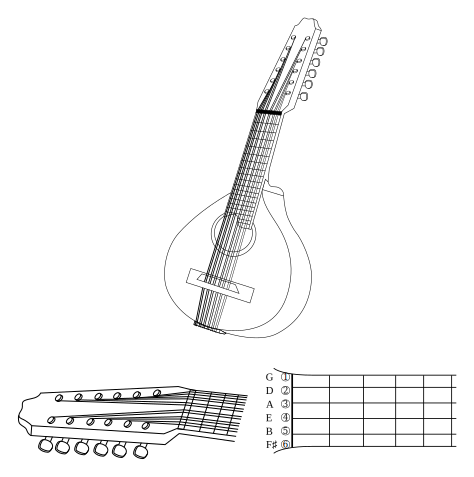
\includegraphics[height=5cm]{img/bandola.png}
\caption[Description of a Colombian Andean Bandola]{Upper image: Colombian Andean Bandola. Lower image: Pitch for each string. From top to bottom in fingerboard strings are tuned in: G, D, A, E, B, F$\sharp$}
\label{Bandola}
\end{figure}

\begin{table}[htb]
\centering
\begin{tabular}{|c|c|c|c|c|c|c|}\hline
\multicolumn{7}{|c|}{\vphantom{\LARGE Ap} Frequencies of tuning for the open strings}\\ \hline\hline
 & G4& D4 & A3 & E3 & B2 & F$\sharp$ 2\\ \hline
Hz & 783.99 & 587.33 & 440 & 329.63 & 246.94 & 185 \\ \hline
\end{tabular}
\caption{Frequency values that correspond to the tuning of open strings in the C-Bandola}
\label{StringTuning}
\end{table}  

Sources of sound in instruments could be of mechanical, acoustical or electrical type. For instance, vibrations of strings, bars, membranes, plates, air in a tube and synthesized sounds. Even sources could be collective coupled vibrators, in other words, a complex system \cite{Rossing}. Related to this fact, instrument analysis is classified according the type of source or sound production. This will indicate the phenomenon involved in each case, and thus, the useful mathematical formulation.

String instruments are a particular case of classification, which commonly, not only involve string vibration in an instrument, but also coupled plates, bars and air oscillations. Violins, guitars and bandola in C are examples in this category and many works have been devoted, at least for violins and guitars, to study their behavior as complex system \cite{Rossing,Christensen, Christensen3, Caldersmith1, Dickens1, Firth1}.

For simplicity, complex systems are divided in subsystems. As an exponent, the phenomena involved in guitars sound production will be presented to distinguish two main subsystems: the first composed by strings, bridge and top plate and the second composed by guitar body parts. Due to the great similarity of guitar and bandola, this example constitutes an excellent description to illustrate physical behavior of bandola in C.

In Figure \ref{GuitarScheme}, a scheme similar to one presented in \cite{Rossing} shows the frequency range in which each subsystem play significant role. From this figure, guitar behavior can be described  as follows: At low frequency, guitar transmits vibrations through the bridge to the top plate, which displaces fluid inside the cavity and induces pressure changes that cause sound hole radiation. Vibrational energy is also transmitted to back plate via both the ribs and air cavity pressure changes. At high frequency, most of the sound is radiated by top plate and the role of the bridge becomes more relevant.  

\begin{figure}[h]
\centering
\includegraphics[height=4cm]{img/GuitarScheme.png}
\caption{Scheme of guitar subsystems according to frequency response}
\label{GuitarScheme}
\end{figure}

This work will treat specifically the analysis of modal coupling at low resonances in the C-Bandola body and hence, the coupling between plates and the enclosed air. 

\section{The Coupled System}

While studying physical behavior of systems, one can find frequently a system linked to others (one or more) where its description depends on the simultaneous description of the others. Therefore, an independent solution is impossible without the parallel solutions of the rest. Such systems are called coupled and the way they interact will determine the coupled system behavior.

This section describes how the fluid-structure coupling is usually treated in a FEM analysis, a topic that concerns us for understanding and solving the problem proposed: the coupling between vibrations of the enclosed air and the plates of a Colombian C-Bandola. Here also will be exposed two simple models of coupled oscillators proposed by Christensen and Vistisen in \cite{Christensen, Christensen3}, where the enclosed air in a guitar and its plates are represented each by an individual oscillator. Basically, the use of these two coupling models will be useful as reference for numerical models and also for numerical results which must reflect predictions of coupling models and will provide further understanding since extended bodies can be modeled.

\subsection{Fluid-structure coupling}

Dynamic fluid-structure interaction can be followed when the motion of the structure induces pressure changes on the fluid (which doesn't penetrate the structure) and produces fluctuating motions. As the fluid moves, the varying pressure field loads the structure and its motion is modified. Thus, the process starts again. Considering the dynamic equations form for structures and the Helmholtz equation for acoustic problems, the expressions for a fluid-structure coupling are reached through Galerkin's variational method (``the weak form") which is useful in finite element method formulation. The coupling is presented using a discrete form of the previous resulted terms.

The weak form for solids can be presented as
\begin{equation}
\int_{\Omega_s} \delta \mathbf{u^T}(\rho_s \ddot{\mathbf{u}}+\mu \dot{\mathbf{u}}+ \mathbf{S^TDSu}-\mathbf{b}) d\Omega - \int_{\Gamma} \delta \mathbf{u^T}\bar{\mathbf{t}} d\Gamma = 0, 
\label{WeakSolid}
\end{equation}
where $\mathbf{u}$ and $\delta \mathbf{u^T}$ are the displacement vector and its variation, the superscript $T$ denotes the transpose; $\dot{\mathbf{u}}$ and $\ddot{\mathbf{u}}$ are the first and second time derivative of displacement vector. $\rho_s$ is the density of the solid, $\mu$ a damping constant, $\mathbf{S}$ is a linear differential operator, $\mathbf{D}$ the elasticity matrix containing the material properties and $\bar{\mathbf{t}}$ is the surface traction defined as
\[
\bar{\mathbf{t}}=-p\mathbf{n_s}= p\mathbf{n}.
\]
Above equation takes a positive pressure in compression and the outward normal to the solid $n_s=-n$. The traction integral in Eq. \ref{WeakSolid} is now expressed as
\[
\int_{\Gamma_t} \delta \mathbf{u^T} \bar{\mathbf{t}} d\Gamma = \int_{\Gamma_t} \delta \mathbf{u^T n}p d\Gamma.
\]

Since the fluid is coupled with the motion of the structure, the acceleration of the fluid particle is equal to the acceleration of the structure in the region of contact. Considering this, the weak form for the acoustic wave is
\begin{equation}
\int_{\Omega_f} \biggr[\delta p \frac{1}{c^2}\frac{\partial^2p}{\partial t^2}+(\nabla \delta p)^T (\nabla p) \biggr] d\Omega + \int_{\Gamma_1} \delta p \rho_0 \mathbf{n^T} \ddot{\mathbf{u}} d\Gamma = 0,
\label{WeakFluid-Bcond1}
\end{equation}
where $p$ and $\delta p$ are the pressure and its variation, $c$ is the sound velocity in the fluid, $\rho_0$ is the fluid density in the hydrostatic state and $\nabla$ is the Gradient. $\Omega_f$ and $\Omega_s$ are the fluid and structure domain, and $\Gamma$ is the boundary part where boundary conditions must be specified. It can be observed that both weak forms for fluid and solid depend on a variable defined in the other coupled phenomenon. This indicates the mutual dependence, i.e., the coupling.

In Eq.\ref{WeakFluid-Bcond1} and Eq.\ref{WeakSolid}, pressure and displacement vectors $p$ and $u$ will be approximated to discretize the system. For this, a shape function is proposed in order to fix pressure and displacement values in a specific domain. This can be expressed as
\begin{eqnarray*}
p & \approx & \hat{p}= N_p\tilde{p}\\
u & \approx & \hat{u}= N_u\tilde{u},
\end{eqnarray*}
where $\tilde{p}$ and $\tilde{u}$ are the vectors of values for pressure and displacement at every point defined in the domain and $N_p$ and $N_u$ are appropriate shape matrices that fix the values at the points in the domain. 

Discretization applied to fluid equation in Eq.\ref{WeakFluid-Bcond1} yields
\begin{equation}
S\ddot{\tilde{p}}+ H\tilde{p}+\rho_0 Q^T \ddot{\tilde{u}}+q = 0,
\label{DiscreteFluid}
\end{equation}
where $q$ is an included source term and
\begin{equation}
\left.
\begin{aligned}
S & = \int_\Omega N^T_p \frac{1}{c^2} N_p d\Omega \\ %\int_{\Gamma_3} N^T_p \frac{1}{g} N_p d\Gamma\\
%\tilde{C} & = \int_{\Gamma_4} N^T_p \frac{1}{c} N_p d\Gamma\\
H & = \int_\Omega (\nabla N_p)^T \nabla N_p d\Omega\\
Q & = \int_{\Gamma_t} N^T_u \mathbf{n} N_p d\Gamma
\end{aligned}
\right\}
\label{Qterm}
\end{equation}

Similarly, the discrete structural problem becomes
\begin{equation}
M\ddot{\tilde{u}}+C\dot{\tilde{u}}+K\tilde{u}-Q\tilde{p}+f=0,
\label{DiscreteSolid}
\end{equation}
where
\begin{eqnarray*}
M & = & \int_\Omega N^T_u \rho_s N_u d\Omega\\
C & = & \int_\Omega N^T_u \mu N_u d\Omega\\
K & = & \int_\Omega B^T D B d\Omega\\
q & = & -\int_\Omega N_u b d\Omega.
\end{eqnarray*}
$B= SN_u$ and $Q$ is identical to Eq. \ref{Qterm}.

If free vibrations are considered and all forces and damping terms are omitted, Eq.\ref{DiscreteFluid} and Eq.\ref{DiscreteSolid} can be written as
\[
\begin{bmatrix}
M & 0\\
\rho_0 Q^T & S
\end{bmatrix}
\begin{Bmatrix}
\ddot{\tilde{u}}\\ \ddot{\tilde{p}}
\end{Bmatrix}
+\begin{bmatrix}
K & -Q\\
0 & H
\end{bmatrix}
\begin{Bmatrix}
\tilde{u}\\ \tilde{p}
\end{Bmatrix} = 0
\]
This is the system of equations that represents our fluid-structure interaction problem. For an eigenvalue problem, it is observed that the system is not symmetric and standard eigenvalue extraction methods are not directly applicable. However, the system is positive semidefinite and it is physically clear that eigenvalues are real and free vibration modes exist.
 
\subsection{Simple model of coupled oscillators}

Modal coupling analysis at low resonances in a bandola can be performed by assuming a coupling model for resonance box. Reported works on the subject \cite{Rossing1, Meyer, Meyer2, Rossing, Rossing3, Christensen, Christensen3, Caldersmith1, Dickens1, Firth1} commonly start with the analysis of two  simple coupling models, each with two and three coupled oscillators respectively. For instance, Meyer, Rossing and Christensen \cite{Rossing1, Meyer, Christensen3} describe that three coupled oscillators: top plate, enclosed air and back plate, produce the first three modal frequencies of a classical guitar resonance box which correspond to combination modes. Considering works in \cite{Meyer2, Rossing3, Christensen}, these authors also reported that a model with two oscillators: top plate and enclosed air, will predict the first two resonances.

According to above ideas and taking in mind that guitars are the closest acoustical reference of bandolas, numerical models that reflect these coupled systems are proposed for modal coupling analysis. Thus, numerical solutions could describe dynamic behavior in the bandola at its first two or three resonances for each case.

\subsubsection{Coupling between top plate and enclosed air.}

Based on the model presented by Christensen and Vistisen in \cite{Christensen}, the coupling between top plate and enclosed air is presented on the basis of Newtonian equations of motion. The model consider the interaction of resonances of two oscillators: Helmholtz resonance and the fundamental top plate resonance. The air inside the cavity vibrates somehow like a Helmholtz resonator for the first mode. In this case, this resonator consist of an air piston in the sound hole, oscillating against the stiffness of the air in the cavity. The fundamental top plate mode in a guitar is characterized by symmetrical variation of amplitude over the lower bout of the guitar \cite{Jansson:GuitarModes}, hence, the model consider this fundamental resonance assuming a simple harmonic oscillator consisting of a plate mass and a piston area, together with a spring stiffness. The back plate is assumed rigid. Figure \ref{Top-Air} illustrates the model.

\begin{figure}[h]
\centering
\includegraphics[height=4cm]{img/Top-Air.png}
\caption{Coupling model of resonance box of two oscillators presented by Christensen and Vistisen}
\label{Top-Air}
\end{figure}


Equations of motion for the system of two coupled oscillators are:
\begin{eqnarray}
m_{p}\ddot{x}_p & = & - k_p x_p  + A \Delta p
\label{EqPlate}\\
m_{a}\ddot{x}_a & = & S \Delta p,
\label{EqAir}
\end{eqnarray}
where $\Delta p  = - \mu \Delta V$, $\mu= c^2 \rho_a / V$, $\Delta V  =  A x_p + S x_a$ and
\begin{eqnarray*}
& x_p \quad  &\text{the displacement of top plate piston}\\
& x_a \quad &\text{the displacement of air piston}\\
& m_p \quad &\text{the plate mass}\\
& m_a \quad &\text{the air piston mass}\\
& k_p \quad &\text{the spring stiffness}\\
& A \quad &\text{the equivalent piston area of top plate}\\
& S \quad &\text{the area of soundhole}\\
& c \quad &\text{the sound velocity in air}\\
& \rho_a \quad &\text{the density of air}\\
& V \quad &\text{the cavity volume}
\end{eqnarray*}
Assuming $x_p=A_p e^{i\omega_p t}$ and $x_a=A_a e^{i\omega_h t}$ in E.q.\ref{EqPlate} and E.q.\ref{EqAir} and using a matrix-vector form, solution of the system is found for the characteristic polynomial:
\begin{equation}
\left( \omega^2 - \frac{k_p + \mu A^2}{m_p} \right) \left( \omega^2 - \frac{\mu S^2}{m_a} \right) - \frac{(\mu SA)^2}{m_p m_a} =0.
\label{2Poly}
\end{equation}
It can be noted from E.q.\ref{EqPlate} and E.q.\ref{EqAir} that resonance frequencies for both separate systems (plate and piston air) $\omega_p$ and $\omega_h$ respectively, are:
\begin{eqnarray*}
\omega^2_p = \frac{k_p + \mu A^2}{m_p}\\
\omega^2_h = \frac{\mu S^2}{m_a},
\end{eqnarray*}
with $\omega^4_{ph}=(\mu SA)^2/m_p m_a$ as a coupling frequency, E.q.\ref{2Poly} yields:
\begin{equation}
(\omega^2 - \omega^2_p)(\omega^2 - \omega^2_h)- \omega^4_{ph} =0,
\end{equation}
An important relation can be given by summing the roots of this system of two oscillators:
\begin{equation}
\omega_{1}^2 + \omega_{2}^2 = \omega^2_p + \omega^2_h.
\label{Combination2}
\end{equation}
Above equation says that square sum of the resonance frequencies in the coupled system equals the square sum of resonances frequencies in the uncoupled system.\\

The model presented by Christensen and Vistinsen is validated through mobility and sound radiation measurements that confirm the great approach to guitar dynamic behavior at the first two resonances. As they mentioned \cite{Christensen}, ``the only condition for establishment of a coupling is that the Helmholtz resonance is present and that the vibration of the top plate (plus back plate eventually) generates a net volume displacement". Therefore, the behavior of bandola at the first two resonances is assumed to be described by this model, and the use of FEM will give a wider scope since it considers an extended body which allows detailed information at every point.

\subsubsection{Coupling between top plate, enclosed air and back plate.}

The influence of the back plate is modelled by introducing another piston with effective area $B$ and mass $m_b$ which acts against a spring of stiffness $k_b$, as described by Christensen \cite{Christensen3}. Motion of any piston causes pressure changes inside the cavity and will affect the motion of the other two pistons. The system of coupled pistons is given in Figure \ref{Top-Back-Air}.

\begin{figure}[h]
\centering
\includegraphics[height=5cm]{img/Top-Back-Air.png}
\caption{Coupling model of resonance box of three oscillators presented by Christensen}
\label{Top-Back-Air}
\end{figure}

The equations of motion for the three pistons in the coupled system are:
\begin{eqnarray}
m_{p}\ddot{x}_p & = & - k_p x_p  + A \Delta p
\label{EqPlate1}\\
m_{a}\ddot{x}_a & = & S \Delta p
\label{EqAir1}\\
m_{b}\ddot{x}_b & = & - k_b x_b  + B \Delta p,
\label{EqBack1}
\end{eqnarray}
where $x_b$ is the displacement of back plate piston.
$\Delta p$, as before, is the pressure change in the cavity resulting from movements of the pistons. Thus,
\begin{eqnarray*}
\Delta p & = & -\mu \Delta V\\
\Delta V & = & A x_p + S x_a + B x_b
\end{eqnarray*}
Again, it is assumed $x_p=A_p e^{i\omega_p t}$, $x_a=A_a e^{i\omega_h t}$ and $x_b=A_b e^{i\omega_b t}$ for equations in Eqs.\ref{EqPlate1}-\ref{EqBack1}. Thus, it can be identified, as in the model of two oscillators, the resonance frequencies of separate systems and the coupling frequencies.

Using the matrix-vector form, it can be found the characteristic polynomial and its roots. It is shown, by summing the roots, that it is also held the relation where the square sum of coupled resonance frequencies is equal to the sum of uncoupled resonance frequencies. Thus,
\begin{equation}
\omega_{1}^2 + \omega_{2}^2 + \omega_{3}^2 = \omega^2_p + \omega^2_h + \omega^2_b.
\label{Combination3}
\end{equation}
Meyer \cite{Meyer2} was the first one to give a detailed technical description for the three-oscillators system. He showed that the effect of back plate is to lower $\omega_1$ and $\omega_2$ and to split $\omega_2$ in two resonances yielding $\omega_3$.

This model is used for description of bandola behavior at the first three resonances, where again the use of FEM will give a wider scope. It was observed that coupled modes are expressed in terms of uncoupled modes, so, numerical models for separate oscillators (of each model) are proposed for analysis in order to appreciate, through comparison, their participation in coupled modes.

An useful detail for analysis can be noted in coupling frequency terms. These terms are ratios of the piston areas and the effective mass of oscillating pistons, with more terms for the case of three oscillators. It can be infer of this fact that a weak or strong coupling will depend on this ratios.

\section{Numerical Model Considerations}

\subsection{Material Properties}

Acoustic waves are assumed to propagate in an inviscid fluid with small amplitudes of vibration, negligibly density variations and negligibly convective effects. Wave propagation will thus depend only on fluid density $\rho_a$ and its bulk modulus $K_s$. For air, using the relation $c= \sqrt{\frac{K_s}{\rho_0}}$, the values can be specified as follows:
\begin{eqnarray*}
\rho_a & = & 1.18 \text{kg/m}^3\\
c & = & 343 \text{m/s} 
\end{eqnarray*}

Moreover, Bandola's plates are made of wood, an orthotropic material which according to the way it was extracted from the tree, could present transverse isotropy. For plates of musical instruments transverse isotropy is common and their material properties are thus specified through five elastic values: Young's modules $E_x$ and $E_y$, Poisson's ratio $\nu_{xy}$, shear modulus $G_{xy}$ and the plate material density $\rho_p$. Although orthotropic properties can be introduced in numerical models, dynamic expressions for plates could be simplified by considering isotropic properties which also simplify numerical computing.\\

The modal analysis proposed in this work is dedicated to study the coupling phenomenon at low resonances, and simple numerical models are pursued in order to ease monitoring the influence of some specific model parameters. The effect of orthotropy over coupling won't be considered as analysis subject, therefore, plates material will be modelled as an isotropic material.\\

For isotropy, elastic values of \textit{Young's Modulus} and \textit{Poisson's ratio} are defined through the geometric mean of properties presented for spruce in \cite{J.Torres1} and rosewood in \cite{Elejabarrieta}. The elastic properties that were used for the average are presented in Table \ref{OrthoMat}. Wood densities are also presented in this table. The averaged values for isotropic plates are presented in Table \ref{IsoMat}.  

\begin{table}[htb]
\centering
\begin{tabular}{|c|c|c|c|c|c|}\hline
\multicolumn{6}{|c|}{\vphantom{\LARGE Ap} Material with transverse isotropy}\\ \hline\hline
 & $\rho_p \quad (kg/m^3)$ & $E_x$ (GPa) & $E_y$ (GPa) & $\nu_{xy}$ & $G_{xy}$ (GPa)\\ \hline
Top plate (Spruce) & 330 & 0.66 & 6.6 & 0.003 & 0.77 \\ \hline
Back Plate (Rosewood) & 775 & 2.2 & 16 & 0.05 & 1.1 \\ \hline
\end{tabular}
\caption{Elastic properties for material with transverse isotropic}
\label{OrthoMat}
\end{table}

\begin{table}[htb]
\centering
\begin{tabular}{|c|c|c|}\hline
\multicolumn{3}{|c|}{\vphantom{\LARGE Ap} Averaged isotropic material}\\ \hline\hline
 & $E$ (GPa) & $\nu$ \\ \hline
Top plate (Spruce) & 2.08 & 0.01 \\ \hline
Back Plate (Rosewood) & 5.93 & 0.13 \\ \hline
\end{tabular}
\caption{Elastic properties for isotropic material.}
\label{IsoMat}
\end{table}

\subsection{CAD Models and analysis considerations}


\subsubsection{CAD Models}

CAD models were designed using SolidWorks\textsuperscript{\textregistered}. Figure \ref{CADTopPlate} presents CAD model for top plate which consists of a drop-shaped plane surface. Dimensions are specified in Figure \ref{PlateDimensions}.\\

As it was mentioned, simple models are pursued and hence, fan bracing, harmonic bars, bridge and sound hole reinforcement are not considered. These parts of the bandola, at low resonances, are expected to increase mass and stiffness without changing the shape modes.\\

\begin{figure}[h]
\centering
\includegraphics[height=4cm]{img/CADTopPlate.png}
\caption{CAD model for Top plate}
\label{CADTopPlate}
\end{figure}

\begin{figure}[h]
\centering
\includegraphics[height=5cm]{img/bandolaFrontarea.pdf}
\caption{Dimensions of modelled plates}
\label{PlateDimensions}
\end{figure}

Figure \ref{CADBackPlate} presents CAD model for back plate which also consists of a drop-shaped plane surface. Dimensions are the same for top plate. \\

\begin{figure}[h]
\centering
\includegraphics[height=3.5cm]{img/CADBackPlate.png}
\caption{CAD model for Back plate}
\label{CADBackPlate}
\end{figure}

It was stated that the air inside the cavity vibrates at the first mode almost as a Helmholtz resonator. This assumption is not so simple because of the geometry of the instrument and also because the cavity walls are not completely rigid. Additionally, the concept of "length of the neck" does not refer exactly to a length determined by either end of the neck. In guitars, for example, it could be thought that the length of the plug of the air is given by top plate thickness, however, practice have shown that an extra volume both inside and outside moves with the air in the neck due to the inertia of the oscillating piston when it gets to its original position. This event is called the \emph{end effect} and the correction that should be applied in order to consider it is related to and of similar size to the diameter of the hole, so the mass of air is substantial. Applying the the correction used for guitars, the effective length of the "plug" of air of the bandola will be about 1.7 times the radius of the hole.\\

%which is given by top plate thickness (3mm).
The CAD model of enclosed air should represent the enclosed volume of air together with the effective length of the resonator's neck. The model presented in Figure \ref{CADBody} could represent not only the above ideas, but also the complete body, formed by surface planes for plates and enclosed volume of air, which is useful for coupling the systems. The ribs have a depth of 10cm as specified.

\begin{figure}[h]
\centering
\includegraphics[height=4cm]{img/CADBody.png}
\caption{CAD model for Bandola's resonance box}
\label{CADBody}
\end{figure}

\subsubsection{FEA Considerations}

Simulations were executed using the commercial software ANSYS\textsuperscript{\textregistered} in a range of analysis of 0-800Hz, both for separate (top-plate, back-plate, enclosed air) and coupled systems. Boundary conditions are imposed in each case.\\

Separate top and back plates are assumed to vibrate clamped at the edge, i.e., the transverse displacement function and its slope equal to zero. The analysis of plates was performed using the element SHELL281 whose formulation is based on the Mindlin-Reissner theory. For the enclosed air, the pressure at the external transverse area of the sound hole equals the atmospheric pressure. This characteristic allows the air to move in and out the cavity as in a Helmholtz resonator; the walls are considered rigid. The element FLUID220 was used for meshing the air, an element based on governing equation for acoustics, namely the 3-D wave equation, and also takes into account the coupling of acoustic pressure and structural motion at the interface.\\

For the coupled system of top plate-enclosed air, Bandola's top plate and back plate are clamped to the ribs and they enclose the air; back plate is considered rigid but top plate vibration couples the system. The enclosed air has the same boundary conditions as in the separate model but only the top plate moves. The coupling condition is present over the top plate-air interface and states that normal to the interface, fluid particle accelerations are equal to plate accelerations. The coupled system of top plate-enclosed air-back plate has the same conditions presented above but now, back plate can vibrate clamped at the edge and the coupling condition is also specified for back plate-air interface.





\section{Results}

\subsection{Modal analysis of uncoupled elements.}

The six lowest modes of vibration of bandola's top and back plate are presented in Figures \ref{TopPlateModes} and \ref{BackPlateModes}, where each mode is identified with the label $(m, n)$ that refers to the number $m$, $n$ of antinodal areas in the $x$ and $y$ directions respectively. Initials "T" for top plate and "B" for back plate that begin the mode label are used to specify the modes for each plate. Colored bar indicates the scale of contours displacement, ranging from blue, the minimum displacement, to red, the maximum displacement. These displacements are not an absolute quantity since each mode is normalized separately, however, their importance lies in the relation between the different contours (amplitudes) in the plate.\\

\begin{figure}[h]
\centering
\includegraphics[height=4cm]{img/TopPlateModes.png}
\caption{Simulated modes of vibration of the top plate.}
\label{TopPlateModes}
\end{figure}

\begin{figure}[h]
\centering
\includegraphics[height=4cm]{img/BackPlateModes.png}
\caption{Simulated modes of vibration of the back plate.}
\label{BackPlateModes}
\end{figure}

According to the material properties of each wood, frequency values for back plate modes are higher than those for top plate. Rosewood is a hardwood and hence, higher frequencies were expected. By comparing the frequencies with those for open strings in Table \ref{StringTuning}, it can be observed that calculated frequencies of the plates are within the sound register of bandola. This fact could mean that material properties used for analysis are in a good range of approximation. Despite of this, it is known that fan bracing and harmonic bars have the effect of increase resonance frequencies of the plates and thus, if numerical models had considered fan bracing, harmonic bars or any structural reinforcement, the modal frequencies would have been higher. Something similar happens in classical guitars \cite{Rossing}, where first top and back plate frequencies, usually 183Hz and 204Hz respectively, are far enough from the lowest tuning frequency of open strings, which is 82Hz.\\

Analyzing the resulted mode shapes for the bandola's plates, it can be confirmed, like in guitars, that the fundamental modes (1,1) are characterized by symmetrical variation of amplitude over the bout of the bandola. This result supports the assumption of coupling models based on \cite{Christensen, Christensen3}, where these first modes of the plates are modelled as simple harmonic oscillators that represent the displacement of the mode effective mass. Besides the fundamental modes, the others can be identified according the experimented stresses, i.e., modes (2,1) and (3,1) are recognized as "transverse flexural modes", modes (1,2) and (1,3) are the "longitudinal flexural modes", and the mode (2,2) is called the "shear mode".

Figure \ref{AirModes13} shows the obtained modes for the air in the cavity. This three lowest modes are identified as the air modes A0, A1, A2. Colored bar indicates the scale of contours pressure, ranging from blue, the minimum pressure, to red, the maximum pressure.

\begin{figure}[h]
\centering
\includegraphics[height=5cm]{img/AirModes13.png}
\caption{Air modes A0, A1 and A2.}
\label{AirModes13}
\end{figure}

Air mode A0 is known as the Helmholtz resonance and according to the coupling models, it is of great importance for bandola's dynamic response at low frequencies since it couples the system. A pure Helmholtz resonator is characterized by a maximum constant pressure inside the cavity (that acts as an air cushion) and a pressure variation in the region of the neck that drives the oscillating piston of air. Considering this, the mode A0 presented in Figure \ref{AirModes13} indicates that air inside of bandola's cavity doesn't behave exactly as a Helmoholtz resonator (though it is very similar) since it presents a little variation in pressure along the cavity. This fact could be explained considering the geometry of the bandola.

It can be observed that the frequency of A0 is considerably far apart from the other modal frequencies, constituting a difference of almost two musical octaves for the nearest mode A1. This characteristic could reflect the great influence of this first mode at the lowest frequencies of the bandola by comparing both the obtained frequencies for plates and bandola's sound register in Table \ref{StringTuning}. Besides A0, A1 shows a transverse pressure distribution and A2 shows a longitudinal pressure distribution.

\subsection{Modal analysis of coupled elements.}

Figures \ref{CoupledModes2a}, \ref{CoupledModes2b} and \ref{CoupledModes2c} show the calculated modes for the system in which the top plate and the air in the cavity interact. Nine modes are presented in the range of 0-800Hz, from these modes several patterns of the uncoupled modes can be identified. The modes are labelled with the initials "TA" that indicate the coupling between Top plate and Air, the scripts "DT", "PF" and "PB" are used to specify the variable plotted, i.e., displacements in top plate, pressure in the front view and pressure in the back view, respectively. Color bar indicates the scale of contours magnitude corresponding to the plotted variable, ranging from blue, the minimum magnitude, to red, the maximum magnitude.

\begin{figure}[h]
\centering
\includegraphics[height=6cm]{img/CoupledModes2a.png}
\caption{Coupled modes of vibration for bandola's resonance box considering the oscillation of top plate and enclosed air. The back plate is assumed to be rigid.}
\label{CoupledModes2a}
\end{figure}

\begin{figure}[h]
\centering
\includegraphics[height=6cm]{img/CoupledModes2b.png}
\caption{Coupled modes of vibration for bandola's resonance box considering the oscillation of top plate and enclosed air. The back plate is assumed to be rigid.}
\label{CoupledModes2b}
\end{figure}

\begin{figure}[h]
\centering
\includegraphics[height=6cm]{img/CoupledModes2c.png}
\caption{Coupled modes of vibration for bandola's resonance box considering the oscillation of top plate and enclosed air. The back plate is assumed to be rigid.}
\label{CoupledModes2c}
\end{figure}

The uncoupled modes calculated for top plate and air have shown that Helmholtz resonance of the air A0 is lower than the fundamental resonance of the top plate T(1,1). As it is exposed in the Figure \ref{CoupledModes2a}, TA(1) and TA(2) present in turn, lower and higher resonances (respectively) compared with those of uncoupled elements. With these results and according to the coupling model of two oscillators, combination of both the fundamental resonance of top plate and the Helmholtz resonance thus give rise to a lower resonance TA(1) and a higher resonance TA(2). From mode shapes, it can also be said that these two coupled modes seem to be efficient radiators since a big area of the bout of the bandola excites the air in front of it. The efficiency of this radiation will also be determined by the phase of piston air and in order to get any information of it, it would be convenient experimental measurements.

Verifying the expression in E.q.\ref{Combination2} it is found that:
\begin{eqnarray*}
\sqrt{f_p^2 + f_h^2} & = & 251.14 \text{Hz}\\
\sqrt{f_1^2 + f_2^2} & = & 273.87 \text{Hz},
\end{eqnarray*}
where the frequency $f=\omega / 2 \pi$. These results are coherent since the percent error, relative to the sum of coupled terms, is 8.3\%. At this point, it would be convenient an experimental validation.

Now, with respect to the other coupled modes in the frequency range, it can be observed throughout the following 7 modes that the combination of the remaining 5 modes of the plate with the other two of the air is presented. As it was expected, the resultant modes are combination of uncoupled modes. In this sense, models more complex could be considered in order to predict more modes, using more oscillators representing every mode in the plate or in the air. A model with nine oscillators, three representing the modes of air inside the cavity and six representing the modes of the top plate, all lying into the same frequency range, would predict the nine calculated coupled modes, also into the same range.

Some global characteristics from of all of the calculated coupled modes can be mentioned. First, the correspondence between uncoupled modes of the top plate and the air in every coupled mode, seems to respond to the longitudinal or transverse disposition of the modes, for instance, transverse top plate modes are usually related to the transverse pressure distribution of mode A1, whereas longitudinal top plates modes are related to the longitudinal pressure distribution of mode A2. The shear mode of the top plate also support this idea since it was related to a pressure distribution that can be described from the combination of both air modes A1 and A2. The other characteristic identified was that coupled modes may be usually driven by those uncoupled modes with the nearest frequency.

Figures \ref{CoupledModes3a}, \ref{CoupledModes3b} and \ref{CoupledModes3c} show the calculated modes for the system in which the top plate, the air in the cavity and the back plate interact. Fifteen modes are presented in the same range, they are labelled with the initials "TAB" that indicate the coupling between Top plate, Air and Back plate, the scripts "DT", "DB", "PF" and "PB" are used to specify the variable plotted, i.e., displacements in top plate, displacements in back plate, pressure in the front view and pressure in the back view, respectively. Colors indicate the scale of contours magnitude as in above figures.

\begin{figure}[h]
\centering
\includegraphics[height=9cm]{img/FSI3a.png}
\caption{Coupled modes of vibration for bandola's resonance box considering the oscillation of top plate, enclosed air and back plate}
\label{CoupledModes3a}
\end{figure}

\begin{figure}[h]
\centering
\includegraphics[height=9cm]{img/FSI3b.png}
\caption{Coupled modes of vibration for bandola's resonance box considering the oscillation of top plate, enclosed air and back plate}
\label{CoupledModes3b}
\end{figure}

\begin{figure}[h]
\centering
\includegraphics[height=9cm]{img/FSI3c.png}
\caption{Coupled modes of vibration for bandola's resonance box considering the oscillation of top plate, enclosed air and back plate}
\label{CoupledModes3c}
\end{figure}

It is observed in Figure \ref{CoupledModes3a} that TAB(1) presents clearly the same mode shapes of T(1,1) and B(1,1) in top and back plates respectively, and that A0 can be easily recognized in the pressure distribution. In this mode, top and back plate vibrate with opposite phases, moving outward and inward and changing considerably the volume of the resonance box. Due to this motion, the air is drawn and expelled from the cavity like a breathing. TAB(1) can be thus called, as in others instruments with resonance box, the "breathing mode" \cite{Pennstate}. Moreover, TAB(2) also presents the shapes of T(1,1) and B(1,1), however, the pressure distribution is very confusing and seems to be highly influenced by both shapes of top and back plate. This time the plates vibrate in phase and thus, the volume of resonance box will change a small amount that depends on the displacement amplitude of the plates, which in this case is greater for top plate. The third coupled mode TAB(3) doesn't have the same problem of identifying the mode that governs pressure distribution: A0 is easily recognized, although a greater pressure variation is present throughout the cavity. The mode shapes in top and back plate are also related to T(1,1) and B(1,1), but now the mode in the back plate present a bigger area of displacement. The motion between both plates is again in opposite phase.

According to the model of coupling with three oscillators, these three lowest modes TAB(1), TAB(2) and TAB(3) show the influence of mainly T(1,1), B(1,1) and A0. In each case, one of the uncoupled modes is dominant over the others, for instance, A0 drives the first coupled mode, T(1,1) drives the second and B(1,1) drives the third. Additionally, these modes seem to be efficient radiators although this is also determined by the phase of piston air. Thus, it would be convenient some experimental measurements in the bandola.

By examining TAB(1), TAB(2) and TAB(3), it can be observed that $f_1<f_h$, $f_2<f_p$ and $f_3>f_b$ where $f_b>f_p>f_h$. In comparison with the two lowest modes TA(1) and TA(2) predicted by the model of two oscillators, the frequencies of TAB(1) and TAB(2) decreased in value as if the effect of considering the back plate was that of an added mass. For guitars, Meyer and Elejabarrieta \cite{Elejabarrieta, Elejabarrieta1} have reported the same behavior when considering the vibration of back plate, however, Christensen \cite{Christensen3} has clarified that the second coupled resonance TAB(2) may be moved either upward (for $f_b<f_p$) or downward (for $f_b>f_p$), depending upon the uncoupled resonance frequencies $f_b$ and $f_p$ of the top and back plate.\\Verifying the expression in E.q.\ref{Combination3} it is found that:
\begin{eqnarray*}
\sqrt{f_p^2 + f_h^2 + f_b^2} & = & 322.66 \text{Hz}\\
\sqrt{f_1^2 + f_2^2 + f_3^2} & = & 351.65 \text{Hz}.
\end{eqnarray*}
These results are consistent since the percent error, relative to the sum of coupled terms, is 8.24\%. With this result, the next step would be an experimental validation, as suggested before.

By observing all coupled modes that were calculated, it is noted that the combination of the uncoupled modes of the plates and the air produces the coupled modes, all lying into the frequency range of 0-800Hz. However, only at the lowest five modes is achieved a strong coupling between the modes of the top plate, the enclosed air and the back plate. The rest of the modes could present a coupling between the top plate and the air alone or almost vibrate separately. This coupling could be thought to have a repulsive effect on the modes with increasing frequency.   

Dynamic response (into a specific frequency range) of a complex structure may be described by the combination of the modes of each substructure (all lying in the same frequency range) \cite{Ewins}, therefore, a model considering fifteen uncoupled oscillators, three representing the modes of air inside the cavity, six representing the modes of the top plate and other six for the modes of the back plate, could predict the fifteen calculated coupled modes. 


\section{Conclusions}

We analyse modal coupling in a Colombian Andean C-Bandola at the frequency range of {0--800 Hz} using the Finite Element Method. First, we described the coupling for two cases using coupled systems with two and three oscillators. This allowed us to validate the numerical analysis developed later, where we verified the coupling between each first uncoupled mode of the top plate, the enclosed air and the back plate, at the lowest two and three resonances (depending on the case) of the coupled systems. The rest of the computed modes were also combinations of other uncoupled modes of each element.

We were able to identify the influence of the uncoupled modes on the resultant coupled modes due to the analysis based on the coupling phenomenon (described with coupled oscillators). In each case one of the uncoupled modes is dominant over the others. As a general conclusion, we remark that the coupled system of top plate-enclosed air presented a strong coupling in all the nine coupled modes. Nevertheless, in the coupled system of top plate-enclosed air-back plate the coupling could be thought to have a repulsive effect on the modes with increasing frequency.

Finally, we found six modes in the range of {0--800 Hz} for the top and back plate and three for the enclosed air. For the coupled systems: top plate-enclosed air and top plate-enclosed air-back plate, we found nine and fifteen coupled modes, respectively, in the same frequency range. Considering that modal parameters can describe the dynamic response of a structure and noting that the models of coupled systems of two and three degrees of freedom predicted the response at the lowest two and three coupled modes, we can say that a model consisting of n degrees of freedom, each one representing one of the normal modes of each uncoupled element existing at the frequency range of {0--800 Hz}, would describe the dynamic behavior of the bandola at the same frequency range. This idea agrees with the theory of modal analysis \cite{Ewins}.

In order to verify the obtained results and get more information about some characteristics of the coupled modes, for instance, the phase of vibration of the air mode and the radiation efficiency, experimental measurements are suggested as further work.


\section{Acknowledgements}

We want to thank Grupo de Investigaci\'on de Mec\'anica Aplicada and also the Research and Teaching Department of Universidad EAFIT, for supporting this project and providing the research facilities

We are also grateful to Professor Ricardo Ruiz Boullosa, Professor Juan Diego Jaramillo and Professor Juan David Cata\~no for their advice, enthusiasm and willingness during this experience with acoustics and computational mechanics.

Finally, we thank the bandolist Jairo Rinc\'on and the luthiers Luis Arbel\'aez and Obdulio Vel\'asquez for providing important information about C-Bandola and its musical panorama.




\bibliography{TrabajoGrado_SERG}
\bibliographystyle{unsrt}

\end{document}


